\ifdefined\COMPLETE
\else
\documentclass[12pt]{article}

\usepackage{amsmath,amsthm,mathtools}
\usepackage{graphicx}
\usepackage{algorithm2e}
\usepackage{thm-restate}
\usepackage{enumitem}

\usepackage{tikz}
\usetikzlibrary{shapes, calc, arrows, through, intersections, decorations.pathreplacing, patterns}
\usepackage[labelformat=simple]{subcaption}
\usepackage[export]{adjustbox}

\newtheorem{theorem}{Theorem}
\newtheorem{definition}[theorem]{Definition}
\newtheorem{thrm}[theorem]{Theorem}
\newtheorem{lem}[theorem]{Lemma}
\newtheorem{corollary}[theorem]{Corollary}

\newcommand{\mb}{\mathbf}
\newcommand{\mc}{\mathcal}
\newcommand\numberthis{\addtocounter{equation}{1}\tag{\theequation}}
\let\oldnl\nl
\newcommand{\nonl}{\renewcommand{\nl}{\let\nl\oldnl}}
\renewcommand\thesubfigure{(\alph{subfigure})}

\DeclareMathOperator*{\argmin}{arg\,min}
\DeclareMathOperator*{\vcdim}{VC-Dim}

\begin{document}
\fi

\section{Restricted Correlation Clustering}
\label{section:RCC}

The results in the previous section show that even under strong promise, correlation clustering is still NP-Hard. Furthermore, it is hard even when given access to an oracle. 

Observe that the requirement of correlation clustering is very demanding. The algorithm is required to find a clustering over the set of all possible clusterings of the domain $X$. In the restricted framework, we change the goalpost slightly. The algorithm is now required to find a clustering $C$ from a class $\mc F$ (of clusterings of $X$). 

\begin{definition}[Restricted correlation clustering (RCC)]
\label{defn:rcc}
Given a clustering instance $(X, d)$, an unknown target clustering $C^*$ and weighting parameter $\mu$. Given a finite class $\mc F$ of clusterings of the set $X$. Find $C \in \mc F$ such that 
\begin{align}
\hat C = \argmin_{C \in \mc F} \enspace L_{C^*}(C)\label{eqn:RCCMain}
\end{align}
\end{definition}

\subsection{Relation to practical applications}
Consider the following scenario from the practitioner's point of view. The practitioner wants to implement correlation clustering. However, he/she knows that the problem is NP-Hard. The practitioner has prior knowledge that one of the many hierarchical clustering algorithms (like single-linkage or max-linkage or average-linkage or complete-linkage) is suitable for his/her dataset\footnote{A nice overview of hierarchical clustering techniques can be found in \cite{maimon2009nhecd}}. A hierarchical clustering algorithm outputs a clustering tree. Every pruning of the tree is a clustering of the original dataset. He/she would now like to know which amongst these clustering algorithms is suitable for his task. After having fixed the algorithm, the practitioner would then  like to know which amongst these many prunings he/she should chose. 

The framework of restricted correlation clustering is applicable in such scenarios. When $\mc F = \{T\}$ where $T$ is a hierarchical clustering of $X$, the goal of RCC is to find the pruning from the tree $T$ which has minimum normalized correlation loss. When $\mc F = \{T_1, \ldots, T_s\}$ where each $T_i$ is a hierarchical clustering of $X$. Then the goal of RCC is to find a pruning with minimum loss amongst the prunings of all the $s$ trees. Note that finding the pruning of the tree is the same as choosing the stopping point criteria when running linkage-based algorithms. Hence, the framework can help us choose the right stopping point for a particular hierarchical clustering algorithm.

If $\mc F = \{C_1, \ldots, C_s\}$ where each $C_i$ is a clustering of the set $X$ then the goal is to find a clustering with minimum loss. Note that $\mc F$ can be any of the examples as defined above or a union of these or some other finite class. 
    
\subsection{Solution strategy}
In the RCC framework, we wish to minimize the loss which depends on the unknown target clustering $C^*$. However, in the absence of any information about $C^*$, there is no hope to find a clustering that minimizes $L_{C^*}$. Hence, to solve the RCC problem we allow the clustering (or learning) algorithm to make queries to a $C^*$-oracle. 
  
Our goal is to calculate quantities $L_{P^+}(C)$ and $L_{P^-}(C)$ (Defn. \ref{defn:normalizedCorrelationLoss}) for each of the clusterings $C \in \mc F$ and then choose the clustering with minimum loss. To calculate both these quantities exactly, for each pair of points in our dataset, we would need to know whether they belong to the same-cluster or different-cluster. In other words, we would need access to the complete ground truth clustering $C^*$. Thus, instead of calculating these two quantities exactly we want to estimate them from a small sample, sampled according to the distributions $P^+$ and $P^-$.  

One strategy to estimate $L_{P^+}(C)$ (and $L_{P^-}$) could be the following. Sample a set $S_+$ (and $S_-$) of pairs using the distribution $P^+$ (and $P^-$). Compute the fraction of mistakes made by each clustering $C$ on $S_+$ (and $S_-$). Using the standard results from vc-dimension theory (Thm. \ref{thm:uniformConvergence}), it is known that using this procedure we can estimate $L_{P^+}$ for each of the clusterings $C \in \mc F$. Similarly, we could also estimate $L_{P^-}$. Using the two estimates, we could then estimate the loss $L_{C^*}$ for each of the clusterings in our class and choose the clustering which has the smallest loss. 

The main problem in this approach is that the distributions $P^+$ and $P^-$ are unknown (as the target clustering $C^*$ is not known). In Section \ref{section:samplingRCC}, we discuss two approaches which (approximately) sample according to these distributions. Then in Section \ref{section:sampleAndQueryComplexity}, we show how these sampling procedures can be used to estimate $L_{C^*}$ for all the clusterings in our class $\mc F$.

\section{Sampling for Restricted Correlation Clustering}
\label{section:samplingRCC}
We first describe the procedure $\mc P_0$ which samples according to $P^-$. Then we describe the procedure $\mc P_1$ which samples approximately according to the distribution $P^+$. 

\RestyleAlgo{ruled}
\SetAlgoNoLine
\LinesNumbered
\SetNlSkip{-0.4em}
\begin{algorithm}
\label{alg:weightedNegPairs}
\caption{Procedure $\mc P_0$ for negative pairs}

\Indp\KwIn{A set $X$ and a $C^*$-oracle.}
\KwOut{$(x, y)$ such that $C^*(x, y) = 0$}

\vspace{0.1in} 
\While{TRUE}{
  Sample $(x, y)$ using $U^2$\\
  \If {$ C^*(x, y) = 0$}{\label{algLine:oracleP1}
  		Output $(x, y)$
	}
}
\end{algorithm}
The procedure samples a pair uniformly at random. Then using the oracle it checks if the sampled pair is negative and terminates if such a pair is found. If not then the process is repeated again. It is an easy exercise (proof in appendix Lemma \ref{lemma:weightedNegUniform}) to see that the procedure $\mc P_0$ samples a pair according to the distribution $P^-$. From the algorithm description it is clear that to sample one negative pair we might need to make more than one query to the $C^*$-oracle. However, since the number of negative pairs is much greater than the number of positive pairs ($\gamma$-skewed) the number of `wasted' queries to the oracle is small. The proof of this result is in the appendix (Lemma \ref{lemma:negQueries}).
   
\subsection{Sampling positive pairs}
\label{section:samplingPositiveLSHable}

We now discuss our procedure $\mc P_1$ which approximates the distribution $P^+$. We show that the procedure samples according to a distribution $T$ which has the following property. The loss $L_{T}$ (Defn. \ref{defn:normalizedCorrelationLoss}) and the loss $L_{P^+}$ for any clustering are close to one another. Hence, estimating the loss of a clustering w.r.t the distribution $\mc T$ also gives an estimate of the loss of that clustering w.r.t $P^+$. Now, we discuss the details of the sampling procedure. 

Our metric $d$ is $(\alpha, \beta)$-informative w.r.t the target clustering $C^*$. That is, amongst all pairs with distance $\lambda$ atleast $\beta$-fraction are positive. A naive sampling strategy is the following. Construct a set $K = \{(x, y): d(x, y) \le \lambda\}$ and then sample uniformly from the set $K$ till a positive sample is found. Since most of the positive pairs have distance $\le \lambda$, this sampling procedure approximates $P^+$ (the uniform distribution over the set of true positives). However, constructing the set $K$ requires $\Theta(|X|^2)$ time. This makes the sampling procedure impractical for many situations. In this section, we will use techniques from locality sensitive hashing (LSH) combined with rejection sampling to develop a sampling procedure $\mc P_1$. We will show that $\mc P_1$ needs only linear pre-processing time (to build the hash maps) and outputs a positive pair sampled approximately according to $P^+$.\\

\noindent\textit{Locality Sensitive Hashing (LSH)}

\vspace{0.02in}\noindent Before we describe our technique, we introduce some relevant notation. A hash function $h: X \rightarrow \mb N$ maps the set $X$ onto the set of natural numbers. Thus, a hashing function partitions the input of size $n$ into $m \le n$ different buckets (or blocks) $B_1, \ldots, B_m$ where each $B_i = \{x : h(x) = b_i\}$ for some $b_i$. Given $(X, d)$, a Locality Sensitive Hashing (LSH) scheme w.r.t the distance metric $d$ (or a similarity metric) aims to partition $X$ into buckets such that `similar' items map to the same bucket with high probability and `dissimilar' items end up in different buckets with high probability. For example, MinHash scheme w.r.t Jaccard similarity measure \cite{broder2000min, broder1997resemblance} is a common LSH-based hashing scheme. Another example is SimHash scheme w.r.t hamming similarity measure \cite{charikar2002similarity}. 


\begin{definition}[LSH-based hashing algorithm]
\label{defn:LSHProperty}
Given a set $(X, d)$ and parameter $s$. An LSH-based hashing algorithm (or scheme) $\mc A$ outputs $s$ different partitions $P_1, \ldots, P_s$ of $X$. Denote $P_i = \{B_{i1}, \ldots, B_{in_i}\}$. We say that $\mc A$ is $(\epsilon, \epsilon')$-tight w.r.t $d$ and $\lambda, \lambda'$ if 

\begin{itemize}
	\item If $d(x, y) \le \lambda$ then  ${\mb P} [ b(x, y) = 1 ]  >  1 - \epsilon$
	\item If $d(x, y) > \lambda'$ then ${\mb P} [ b(x, y) = 1 ] < \epsilon'$
\end{itemize}
where $b(x, y) = 1$ if and only if $x, y$ are together in atleast one of the blocks $B_{ij}$.

Infact, we show that by choosing $s$ (and other parameters) appropriately, we can construct LSH schemes which are $(\epsilon, \epsilon'=s\ln (1+\epsilon))$-tight w.r.t $\lambda$ and $\lambda' = 2\lambda \ln (1+1/\epsilon)$. Thus, for simplicity of notation, we say that $\mc A$ is $\epsilon$-tight w.r.t $\lambda$ to mean that it is $(\epsilon, \epsilon')$-tight w.r.t $\lambda, \lambda'$ as chosen above.
\end{definition}

\noindent Throughout the remainder of this section, we will assume that the hashing scheme satisfies $\epsilon$-tightness. In the appendix, we provide details about why this assumption is justified. However, these results are orthogonal to the current discussion. Hence, we omit it here and only include it in the appendix (Thm. \ref{thm:similarInSame}).  

We now describe our sampling procedure. Let $\mc B := \{P_1, \ldots, P_s\} = \{B_{ij} : 1\le i\le s, 1\le j \le |P_i|\}$ be the set of blocks outputted by the hashing scheme and let $Q := \{(x, y) \in B_{ij}\}$.  We first choose a block $B \in \mc B$ with probability proportional to $|B|^2$ (the number of pairs in the block). Then we sample a pair uniformly at random from this block $B$. Note that this strategy doesn't give us a uniform sample from $Q$. This is because a pair $(x, y)$ may be present in multiple blocks. To get the uniform sample, we reject the pair with probability inversely proportional to $a(x, y)$ (the number of blocks in which $x, y$ are together). This approach based on rejection sampling ensures that we have a uniform sample from $Q$. 

Next, we check if the pair satisfies $d(x, y) \le \lambda$. Note that the LSH-based scheme tries to put similar points in the same bucket, hence the probability of success at this step is `high'. Finally, we check if $C^*(x, y) = 1$. Our sampling procedure $\mc P_{1}$ is described in Alg. \ref{alg:weightedPosPairsHash}. 

\begin{algorithm}[h]
\caption{Sampling procedure $\mc P_{1}$ for positive pairs}
\label{alg:weightedPosPairsHash}
\Indp\KwIn{A set $\mc X$, a hashing algorithm $\mc A$, a $C^*$-oracle and parameter $\lambda$.}
\KwOut{$(x, y)$ such that $ C^*(x, y) = 1$}

\vspace{0.1in}\nonl\textbf{Pre-compute:} \\
	Use an LSH-based hashing scheme $\mc A$ to obtain partitions $\{P_1, \ldots, P_s\}$.\\
	$\mc B := \{P_1, \ldots, P_s\} = \{B_{ij} : 1\le i\le s, 1\le j \le |P_i|\}$.\\

\setcounter{AlgoLine}{0}

\vspace{0.1in}\nonl\textbf{Sampling:} \\
\While{TRUE}{
	Sample a block $B$ from $\mc B$ with probability $\propto |B|^2$.\\
	Sample $(x, y)$ uniformly at random from $B^2$. \\
	Let $a(x, y) = \{(x, y) \in B^2: B \in \mc B\}$. \\
	Sample $u$ uniformly at random from $[0, 1]$.\\
		\If{$u > \frac{1}{|a(x, y)|}$}{ \label{algLine:uCheck}
			\textbf{continue}.
		}
	\If {$d(x, y) \le \lambda$ and $C^*(x, y) = 1$ } {\label{algLine:oracleP22}
			 Output $(x, y)$.
	 }	
}
\end{algorithm}


Thm. \ref{thm:posDistribution} shows that with high probability the procedure $\mc P_{1}$ samples a pair according to a distribution $\mc T$  which approximates $P^+$. 
\begin{restatable}{thrm}{posDistribution}
\label{thm:posDistribution}
Given $(X, d)$, a $C^*$-oracle and parameter $\lambda$. Let $d$ satisfy $(\alpha, \beta)$-informative  w.r.t $C^*$. Let the hashing algorithm $\mc A$ satisfy $\epsilon$-tightness w.r.t $\lambda$. Then with probability atleast $1-\exp\big(\frac{-\epsilon^2(1-\alpha)|X^2_+|}{8}\big)$ (over the randomness in the hashing algorithm), $\mc P_{1}$ samples pairs $(x, y)$  according to distribution $\mc T$ over $X^{[2]}$ such that for any labelling function $C : X^{[2]} \rightarrow \{0, 1\}$, we have that 
\begin{align*}
  &\underset{(x, y) \sim P^+}{\mb P} \big[ C(x, y) = 0 ] -\alpha -\epsilon \le \underset{(x, y) \sim T}{\mb P} \big[ C(x, y) = 0 ] \\
  &\le  (1 + 2\epsilon)(1+2\alpha) \underset{(x, y) \sim P^+}{\mb P} \big[ C(x, y) = 0 ]
\end{align*} 
\end{restatable}

To sample one same-cluster pair, we might need to make more than one same-cluster query to the $C^*$-oracle. Lemma \ref{lemma:posQueries} shows that with high probability, the number of queries made by $\mc P_{1}$ to sample one positive pair is upper bounded by a small constant. 

\begin{restatable}{lem}{posQueries}
\label{lemma:posQueries}
Given set $X$, a $C^*$-oracle and parameter $\lambda$. Let $d$ be $(\alpha, \beta)$-informative w.r.t $\lambda$ and $C^*$. Let $\mc A$ satisfy $\epsilon$-tightness w.r.t $\lambda$. Let $q$ be the number of same-cluster queries made by $\mc P_1$. Then with probability atleast $1-\exp\big(\frac{-\epsilon^2(1-\alpha)|X^2_+|}{8}\big)$ (over the randomness in the hashing algorithm) $$\mb E[q] \le \frac{1}{\beta(1-\epsilon)}$$ 
\end{restatable}

The pre-compute stage uses a hashing algorithm to obtain $s$ different partitions. From the discussion in the appendix (Thm. \ref{thm:hashTimeComplexity}), we its easy to see that this runs in $O(n)$ time. Next, we  analyse the time taken to sample one same-cluster pair.  Thm. \ref{thm:posRuntime} shows that under reasonable assumptions, the time taken is upper bounded by a constant with high probability. 

\begin{restatable}{thrm}{posRuntime}
\label{thm:posRuntime}
Given set $X$, a $C^*$-oracle and parameter $\lambda$. Let $d$ be $(\alpha, \beta)$-informative w.r.t $\lambda$ and $C^*$. Let $\mc A$ satisfy $\epsilon$-tightness w.r.t $\lambda$. 

Define $\lambda' = 2\lambda\log(1+\frac{1}{\epsilon})$ and $\epsilon' = \lceil \log(\frac{1}{\epsilon})\rceil (1+\log(\frac{1}{\epsilon}))$. Let $K = \{(x, y) : d(x, y) \le \lambda\}$ is the set of all pairs of points with distance $\le \lambda$. Similarly, define sets $K_1 = \{(x, y): \lambda < d(x, y) \le \lambda'\}$ and $K_2 = \{(x, y): d(x, y) > \lambda'\}$. Let $|K_1| \le \rho_1|K|$ and $\epsilon'|K_2| \le \rho_2|K|$. Define $\eta := \frac{(1-2\epsilon)\beta}{1+\rho_1+\rho_2}$.

Let $t$ be the time taken to sample one point. Then with probability atleast $1- \exp\Big(\frac{- \epsilon^2 (1-\mu)|X^2_+|}{(4-2\epsilon)}\Big)- \exp\Big(\frac{-\epsilon^2(1-\mu)\rho_2 |K|}{(2-\epsilon)^2}\Big)$ (over the randomness in the hashing algorithm), we have that $$\mb E[t] \le \frac{s^2}{\eta}$$. 
\end{restatable}

\section{Sample and query complexity of RCC}
\label{section:sampleAndQueryComplexity}
In the previous section we saw how to sample (approximately) according to the distributions $P^+$ and $P^-$. We sample a `small' set of true positive (or same-cluster) and true negative (or different-cluster) pairs using our distributions. We then choose the clustering $\hat C \in \mc F$ with the minimum number of mistakes on the sampled pairs. We prove that the true normalized correlation loss $L_{C^*}(C)$ is close to the loss of $\hat C^*$ (the clustering with minimum loss in $\mc F$). Thus, our solution strategy shows that by only having a small amount of information about $C^*$ (making a small number of queries) we can find a clustering which is close (in terms of loss) to the optimal clustering in $\mc F$. We describe this procedure in Alg. \ref{alg:ERM}. 

\RestyleAlgo{ruled}
\SetAlgoNoLine
\LinesNumbered
\SetNlSkip{-0.4em}
\begin{algorithm}[h]
\caption{Empirical Risk Minimization}
\label{alg:ERM}
\Indp\KwIn{$( X, d)$, a set of clusterings $\mc F$, a $C^*$-oracle, parameter $\lambda$ and sizes $m_+$ and $m_-$.}
\KwOut{$ C \in \mc F$}

\vspace{0.1in} 
Sample a sets $S_+$ and $S_-$ of sizes $m_+$ and $m_-$ using procedures $\mc P_{1}$ and $\mc P_0$ respectively.\\
For every $C \in \mc F$, compute
\vspace{-0.1in}\begin{align*}
  &\hat P(C) = \frac{|\{(x, y) \in S_+: C(x, y) = 0\}|}{|S_+|}\\
  &\hat N(C) = \frac{|\{(x, y) \in S_-: C(x, y) = 0\}|}{|S_-|}
\end{align*}

Define $\hat L(C) = \mu \hat P(C) + (1-\mu)\hat N(C)$. \label{algLine:alpha}\\
Output $\argmin_{C \in \mc F} \enspace \hat L(C)$ \label{algLine:ERM}
\end{algorithm}

Thm. \ref{thm:sampleComplexity} analyses the sample complexity of our approach. That is, the number of labelled positive and negative pairs our algorithm needs as input, so that the estimates of the loss based on this sample are close to their true values. We show that as long as the number of sampled pairs are in $O(\frac{\vcdim(\mc F)}{\epsilon^2})$ then our algorithm finds a clustering $\hat C$ which is close to the best clustering in $\mc F$. Here, $\vcdim$ is a combinatorial property which measures how `complex' or rich the class of clusterings is. Note that the number of samples needed is independent of the size of the dataset $X$. 

For common classes, like $\mc F = \{T_1, \ldots, T_s\}$ where each $T_i$ is a hierarchical clustering of $X$, \cite{kushagra2018semisupervised} showed that the $\vcdim(\mc F)$ is in $o(\log s)$. Thus for such classes a small number of samples suffice to find a clustering which is close to the best clustering in $\mc F$.  

\begin{restatable}{thrm}{sampleComplexity}
Given metric space $(X, d)$, a class of clusterings $\mc F$ of $X$ and a threshold parameter $\lambda$. Given $\epsilon, \delta \in (0, 1)$ and a $C^*$-oracle. Let $d$ be $(\alpha, \beta)$-informative w.r.t $C^*$ and $\lambda$ and let $X$ satisfy $\gamma$-skewed property. Let $\mc A$ be the ERM-based approach as described in Alg. \ref{alg:ERM} and $\hat C$ be the output of $\mc A$. If  
\label{thm:sampleComplexity}
\begin{align}
  &m_-, m_+ \enspace \ge a\frac{\vcdim({\mc F}) + \log(\frac{3}{\delta})}{\epsilon^2} 
\end{align}
where $a$ is a global constant then with probability atleast $1-\delta$ (over the randomness in $\mc A$), we have that $$L_{C^*}(\hat C) \enspace\le\enspace \min_{\mc C \in \mc F} L_{C^*}(C) + 3\alpha + \epsilon$$
\end{restatable}
\begin{proof}
Let $T_0$ be the distribution induced by $\mc P_0$ and $T_1$ be the distribution induced by $\mc P_1$. Using Thm. \ref{thm:uniformConvergence}, we know that if $m_+ > a\frac{\vcdim({\mc F}) + \log(\frac{1}{\delta})}{\epsilon^2}$ then with probability atleast $1-\delta$, we have that for all $C$
\begin{align*}
  &|\hat P(C) - \underset{(x,y) \sim T_1}{\mb P}[C(x, y) = 0]| \le \epsilon\\
  \implies &\hat P(C) \le \epsilon + (1+2\epsilon)(1+2\alpha)L_{P^+}(C) \enspace\text{ and}\\
  &L_{P^+}(C) - \mu -\epsilon \le \hat P(C) \numberthis \label{eqn:eHat}
\end{align*}
Note that we obtain upper and lower bounds for $\underset{(x,y) \sim T_1}{\mb P}[h(x, y) = 0]$ using Thm. \ref{thm:posDistribution}. Similarly, if $m_- > a\frac{\vcdim({\mc F}) + \log(\frac{1}{\delta})}{\epsilon^2}$, then with probability atleast $1-\delta$, we have that for all $h$,
\begin{align*}
  &|\hat N(C) - \underset{(x,y) \sim T_0}{\mb P}[C(x, y) = 1]| \le \epsilon\\
  \implies &\hat N(C) \le \epsilon + L_{P^-}(C) \enspace\text{ and } L_{P^-}(C) -\epsilon \le \hat N(C) \numberthis\label{eqn:gHat}
\end{align*}

\noindent Combining Eqns. \ref{eqn:eHat} and \ref{eqn:gHat}, we get that with probability atleast $1-2\delta$, we have that for all $C \in {\mc F}$
\begin{align*}
  \hat L(C) &\le \mu [\epsilon + (1+2\epsilon)(1+2\alpha)L_{P^+}(C)]\\
  &+ (1-\mu)(\epsilon + L_{P^-}(C)) \le L_{C^*}(C) + 7\epsilon + 2\alpha\\
  \text{And} \enspace \hat L(C) &\ge \mu(L_{P^+}(h) -\epsilon - \alpha) + (1-\mu)(L_{P^-}(h) - \epsilon) \\
  &\ge L_{C^*}(C) - \epsilon - \alpha
\end{align*}
Now, let $\hat C$ be the output of $\mc A$ and let $\hat C^*$ be $\argmin_{C \in {\mc F}} L_{C^*}(C)$. Then, we have that with probability atleast $1-2\delta$
\begin{align*}
  L_{C^*}(\hat C) &\le \hat L(\hat C) + \alpha + \epsilon \le \hat L(\hat C^*) + \alpha + \epsilon \\
  &\le L_{C^*}(\hat C^*) + 8\epsilon + 3\alpha 
\end{align*}

Choosing $\epsilon = \frac{\epsilon}{9}$ and $\delta = \frac{\delta}{2}$ throughout gives the result of the theorem,
and this completes the proof of the theorem.
\end{proof}

Finally, we analyse the query complexity of our approach. That is the number of queries that our algorithm makes to the $C^*$-oracle. Our algorithm makes queries during the sampling procedure. We see that to sample $m_-$ negative and $m_+$ positive pairs the number of queries is `close' to $m_+ + m_-$ with very high probability. Thus, the number of `wasted' queries is small.  

\begin{restatable}{thrm}{queryComplexity}[Query Complexity]
\label{thm:queryComplexity}
Let the framework be as in Thm. \ref{thm:sampleComplexity}. With probability atleast $1-\exp\big(-\frac{\nu^2m_-}{4}) - \exp\big(-\frac{\nu^2m_+}{4}\big) - \exp(\frac{-\epsilon^2(1-\alpha)|\mc X_+^2|}{8})$ over the randomness in the sampling procedure, the number of same-cluster queries $q$ made by $\mc A$ is  
$$q \le (1+\nu)\bigg(\frac{m_-}{(1-\gamma)} + \frac{m_+}{\beta(1-\epsilon)}\bigg)$$
\end{restatable}

\begin{proof}
The number of queries made to sample the set $S_g$ is $q_g = m_g$. Let $q_+$ denote the number queries to sample the set $S_+$. Using Lemma \ref{lemma:posQueries}, we know that $\mb E[q_+] \le \frac{1}{\beta(1-\epsilon)}$ with probability atleast $1-\exp(\frac{-\epsilon^2(1-\alpha)|\mc X_+^2|}{8})$ over the randomness in the hashing procedure. Given that the expectation is bounded as above, using Thm. \ref{thm:geometricRV}, we get that $q_+ \le \frac{(1+\nu)m_+}{\beta(1-\epsilon)}$ with probability atleast $1-\exp(\frac{-\nu^2m_+}{4})$. Similarly, combining Lemma \ref{lemma:negQueries} with Thm. \ref{thm:geometricRV}, we get that with probability atleast $1-\exp(\frac{-\nu^2m_-}{4})$, $q_- \le \frac{(1+\nu)m_-}{(1-\gamma)}$.
\end{proof}

\section{VC-Dimension of some common classes of clusterings}
In the previous section, we proved that the sample complexity of learning a class of clusterings $\mc F$ depends upon $\vcdim({\mc F})$. Recall that ${\mc F}$ is the class of labellings induced by the clusterings in $\mc F$. In this section, we prove upper bounds on the VC-Dimension for some common class of clusterings. 

\begin{restatable}{thrm}{VCDim}
Given a finite set $\mc X$ and a finite class $\mc F = \{C_1, \ldots, C_s\}$ of clusterings of $\mc X$.
$$\vcdim({\mc F}) \le g(s)$$ where $g(s)$ is the smallest integer $n$ such that $B_{\sqrt n} \ge s$ where $B_i$ is the $i^{th}$ bell number \cite{bell2010number}. 
\end{restatable}


\noindent Note that $B_{\sqrt n} \in o(2^{n})$. Thus, the $\vcdim$ of a list of clusterings is in $o( \log s)$. Next, we discuss another common class of clusterings, namely hierarchical clustering trees. 

\begin{definition}[Hierarchical clustering tree]
Given a set $X$. A hierarchical clustering tree $T$ is a rooted binary tree with the elements of $X$ as the leaves. 
\end{definition}

\noindent Every pruning of a hierarchical clustering tree is a clustering of the set $X$. A clustering tree contains exponentially many (in the size of $\mc X$) clusterings. Given $\mc F = \{T_1, \ldots, T_s\}$ consists of $s$ different hierarchical clustering trees, the following theorem bounds the VC-Dimension of ${\mc F}$.

\begin{restatable}{thrm}{VCDimT}
Given a finite set $\mc X$ and a finite class $\mc F = \{T_1, \ldots, T_s\}$ where each $T_i$ is a hierarchical clustering over $\mc X$. Then 
$$\vcdim({\mc F}) \le g(s)$$ where $g(s)$ is the smallest integer $n$ such that $\frac{\sqrt n!}{\lfloor \sqrt n/2 \rfloor! \enspace 2^{\lfloor \sqrt n/2 \rfloor}} \ge s $
\end{restatable}


\section{Efficient ERM Learner for hierarchical clustering trees}
\label{section:efficientERM}
\begin{algorithm}
\caption{ERM approach for a hierarchical clustering tree}
\label{alg:ERMTrees}
\Indp\KwIn{A set $X$, a set $ S \subseteq X^2$ labelled according to $C^*$. Let $S_u = \{x: (x, y) \text{ or }  (y, x) \in S\}$. Given a clustering tree $T$ on $S_u$.}
\KwOut{A clustering $\hat C \in T$ which implements the ERM approach over $T$.}

\vspace{0.1in} For every node $\nu$, let $nl(\nu)$ be the leaves which are descendants of $\nu$. For a leaf node $\nu$, $nl(\nu) = \{\nu\}$. \\
Let $\mu_1 = \mu|S_-|$ and $\mu_2 = (1-\mu)|S_+|$. Let $$e(\nu) = \argmin_{C \in T_{\nu}} \mu_1|S_+|\hat P(C) + \mu_2|S_-|\hat N(C)$$ where $T_{\nu}$ is the tree $T$ restricted to the descendants of $\nu$. Let $a(\nu) = \mu_1|S_+|\hat P(C) + \mu_2|S_-|\hat N(C)$ where $C$ is the clustering which assigns all the descendants of $\nu$ to a single cluster. \\
Initialize $e(\nu) = a(\nu) = 0$ for all the leaf nodes $\nu$. \\
\For{all non-leaf nodes $\nu$ (in a bottom-up manner)}{\label{algLine:forNode}
Let $\nu_l$ be left sub-tree and $\nu_r$ the right sub-tree.\\
Initialize $s_a = d_a = 0$.\\
	\For{$(x, y) \in S$}{
	  \If {$x, y \in nl(\nu)$ and $C^*(x, y) = 0$}{
	      $d_a = d_a + 1$.
	  }
	  \If {$!(x \in nl(\nu_l)$ and $ y \in nl(\nu_r))$ and $!(y \in nl(\nu_l)$ and $ x \in nl(\nu_r))$}{\label{algLine:IfCondn}
		\textbf{continue}
	}
	\If {$C^*(x, y) = 1$}{
		$s_a = s_a + 1$.
	}
}
$a(\nu) = d_a$ \label{algLine:all}\\
$e(\nu) = \min \{e(\nu_l)+e(\nu_r)+s_a, a(\nu)\}$ \label{algLine:best}
}
\end{algorithm}

Alg. \ref{alg:ERM} described the general ERM approach to find the `best' clustering for any class $\mc F$ of clusterings. Consider the case when $\mc F = \{C_1, \ldots, C_s\}$ (a finite list of clusterings). Then to implement Alg. \ref{alg:ERM}, we first sample a set $S \subseteq X^2$ and then compute the error of each clustering on this set $S$. Computing the error of a clustering on $S$ takes $\Theta(|S|)$ time. Hence, for finite $\mc F$, the ERM approach can be implemented in time $\Theta(|\mc F| |S|)$. 

Now, let's focus on the case when $\mc F = \{T_1, \ldots, T_s\}$ (a finite set of clustering trees). Each tree $T_i$ can contain exponentially many clusterings. Hence, it is not clear if we can still implement the ERM approach in polynomial-time. Consider the problem of implementing the ERM approach when $\mc F = \{T\}$. The goal is to find the pruning in the tree which minimizes the loss $\hat L$. Given tree $T$, the clustering with the smallest loss is either the clustering which assigns all the points to a single cluster or the clustering with the best loss in $T_l$ (left subtree) concatenated with the clustering with the best loss in $T_r$ (right subtree). We describe our bottom-up approach in Alg. \ref{alg:ERMTrees}. Its easy to see that the running time of the approach is $\Theta(|S|^2)$. 
\section{Evaluation}
\label{sec:evaluation}

\begin{table*}[t]
\centering
\resizebox{\textwidth}{!}{
\begin{tabular}{ |c|c|c|c|c|c|c|c|c|c|c|c|c| } 
 \hline
  &  & \multicolumn{2}{|c|}{\textbf{25, 25 samples}} & \multicolumn{2}{|c|}{\textbf{100, 100 samples}} & \multicolumn{2}{|c|}{\textbf{250, 250 samples}} & \multicolumn{2}{|c|}{\textbf{500, 500 samples}} & \multicolumn{2}{|c|}{\textbf{1000, 1000 samples}} \\ \hline
Clustering & true loss & \# queries & estimated loss & \# queries & estimated loss & \# queries & estimated loss & \# queries & estimated loss  & \# queries & estimated loss \\ \hline
C1 (single) & \textbf{0.06107} & 51 &	0.06 & 204	& 0.025 & 519 &	0.028 & 1023 &	0.024 & 2070 &	0.028 \\ \hline
C2 (complete) &	\textbf{0.04177} &	50 & 0.02 &	210 &	0.005 & 514 &	0.018 &		1024 &	0.016 &		2056 &	0.015   \\ \hline
C3 (weighted) & \textbf{0.03831} &	50 & 0.02 &	203 &	0.015 &	518 &	0.008 &		1027 &	0.016 &		2057 &	0.018  \\ \hline
C4 (average) &	\textbf{0.03489} &	52 & 0.02 &	207 &	0.020 &	519	&   0.008 &		1043 &	0.013 &		2061 &	0.014   \\ \hline
\end{tabular}
}
\caption{Simulated dataset: Impact of number of samples on the loss of the clustering}
\label{tab:exp1}
\end{table*}

\begin{table*}[t]
\centering
\resizebox{\textwidth}{!}{
\begin{tabular}{ |c|c|c|c|c|c|c|c|c|c|c|c|c| } 
 \hline
  &  & \multicolumn{2}{|c|}{\textbf{25, 25 samples}} & \multicolumn{2}{|c|}{\textbf{100, 100 samples}} & \multicolumn{2}{|c|}{\textbf{250, 250 samples}} & \multicolumn{2}{|c|}{\textbf{500, 500 samples}} & \multicolumn{2}{|c|}{\textbf{1000, 1000 samples}} \\ \hline
Clustering & true loss & \# queries & estimated loss & \# queries & estimated loss & \# queries & estimated loss & \# queries & estimated loss  & \# queries & estimated loss \\ \hline
C1 (single) & \textbf{0.11075} & 51	& 0.08 & 208 &	0.055 &		516 &	0.054 &		1031 &	0.041 &		2079 &	0.046 \\ \hline
C2 (complete) &	\textbf{0.37172} &	50 & 0.34 &	204 &	0.315 &	510 &	0.348 &		1035 &	0.334 &		2070 &	0.343   \\ \hline
C3 (weighted) & \textbf{0.29622} &	51 & 0.14 &	203 &	0.260 &	521 &	0.236 &		1037 &	0.239 &		2071 &	0.229  \\ \hline
C4 (average) &	\textbf{0.26877} &	50 & 0.20 &	204 &	0.195 &	518 &	0.188 &		1027 &	0.202 &		2074 &	0.193   \\ \hline
\end{tabular}
}
\caption{Publications dataset: Impact of number of samples on the loss of the clustering}
\label{tab:exp2}
\end{table*}

\begin{figure*}[t]
    \centering
    \begin{subfigure}[t]{0.22\textwidth}
        \centering
        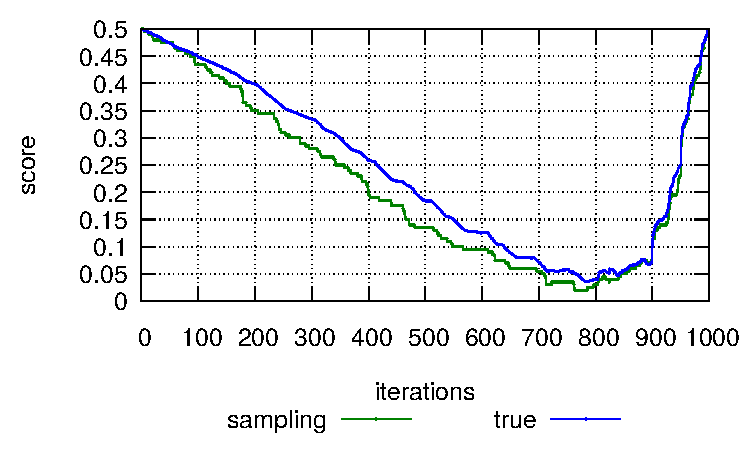
\includegraphics[height=3.2cm, width=4.2cm,valign=t]{figures/plot_simulated_s.pdf}
        \caption{Single linkage}
    \end{subfigure}%
    ~ 
    \begin{subfigure}[t]{0.22\textwidth}
        \centering
        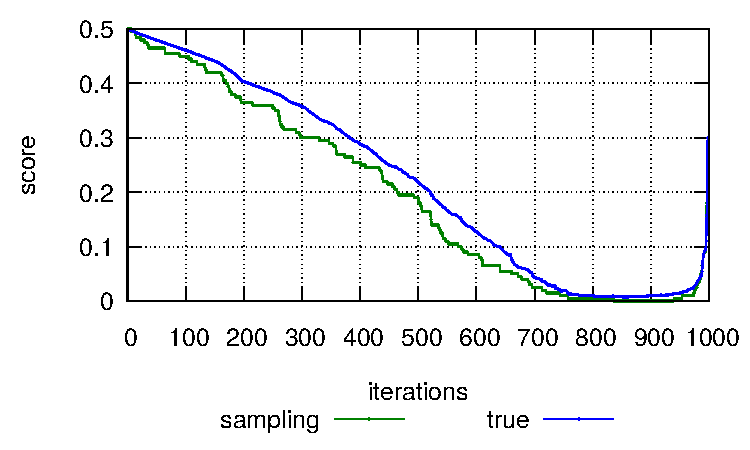
\includegraphics[height=3.2cm, width=4.2cm,valign=t]{figures/plot_simulated_c.pdf}
        \caption{Complete linkage}
    \end{subfigure}
	~
	\begin{subfigure}[t]{0.22\textwidth}
        \centering
        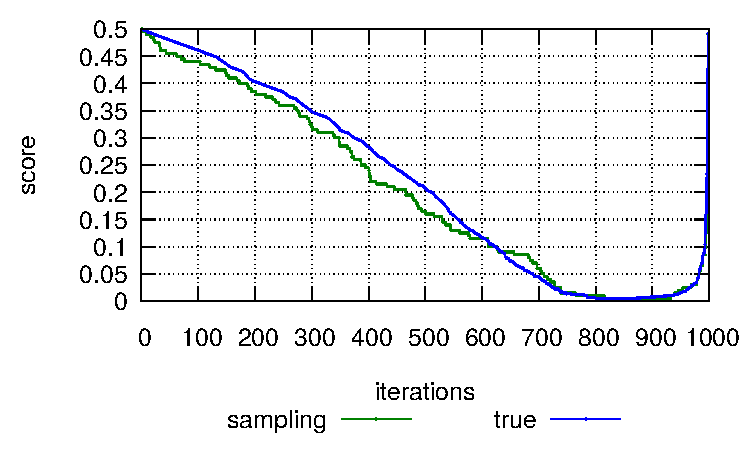
\includegraphics[height=3.2cm, width=4.2cm,valign=t]{figures/plot_simulated_w.pdf}
        \caption{Weighted linkage}
    \end{subfigure}
    ~
	\begin{subfigure}[t]{0.22\textwidth}
        \centering
        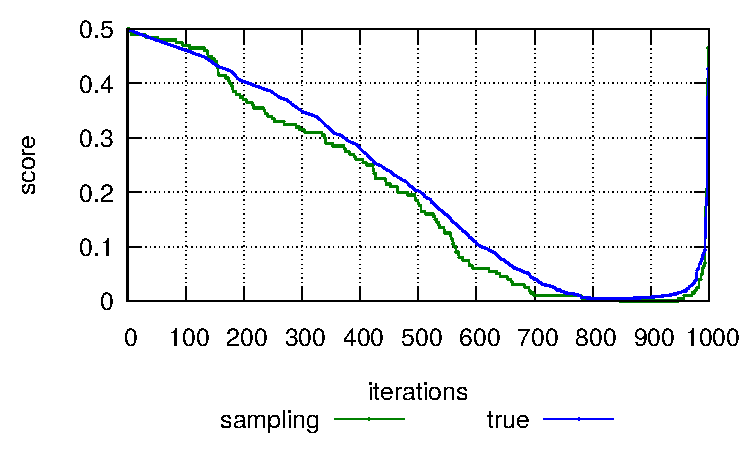
\includegraphics[height=3.2cm, width=4.2cm,valign=t]{figures/plot_simulated_a.pdf}
        \caption{Average linkage}
    \end{subfigure}
    
    \caption{Simulated dataset: Loss reported for every iteration of hierarchical clustering}
    \label{fig:simulated}
\end{figure*}

\begin{figure*}[t]
    \centering
    \begin{subfigure}[t]{0.22\textwidth}
        \centering
        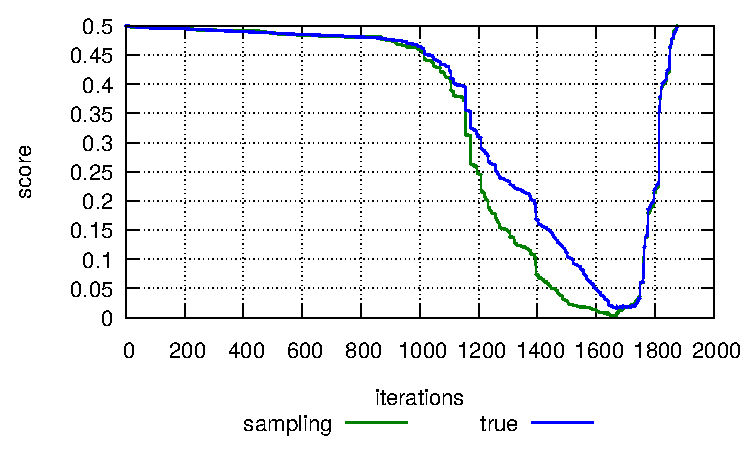
\includegraphics[height=3.2cm, width=4.2cm,valign=t]{figures/plot_real_s.pdf}
        \caption{Single linkage}
    \end{subfigure}%
    ~ 
    \begin{subfigure}[t]{0.22\textwidth}
        \centering
        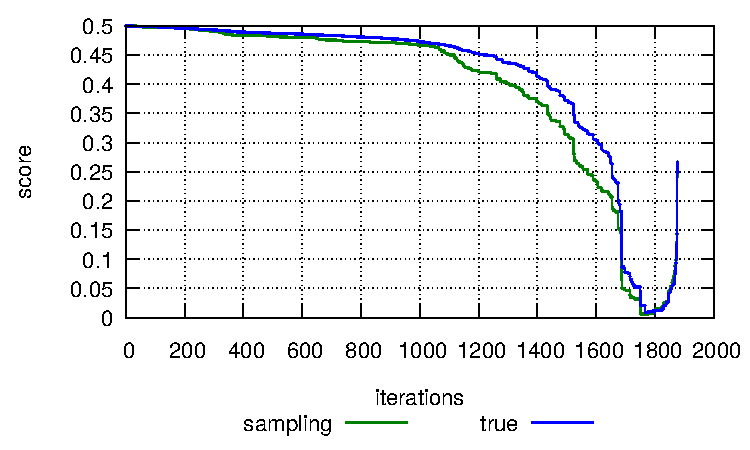
\includegraphics[height=3.2cm, width=4.2cm,valign=t]{figures/plot_real_c.pdf}
        \caption{Complete linkage}
    \end{subfigure}
	~
	\begin{subfigure}[t]{0.22\textwidth}
        \centering
        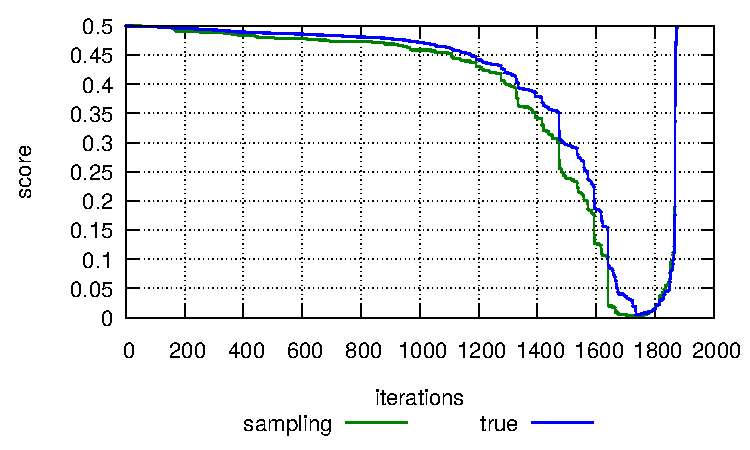
\includegraphics[height=3.2cm, width=4.2cm,valign=t]{figures/plot_real_w.pdf}
        \caption{Weighted linkage}
    \end{subfigure}
    ~
	\begin{subfigure}[t]{0.22\textwidth}
        \centering
        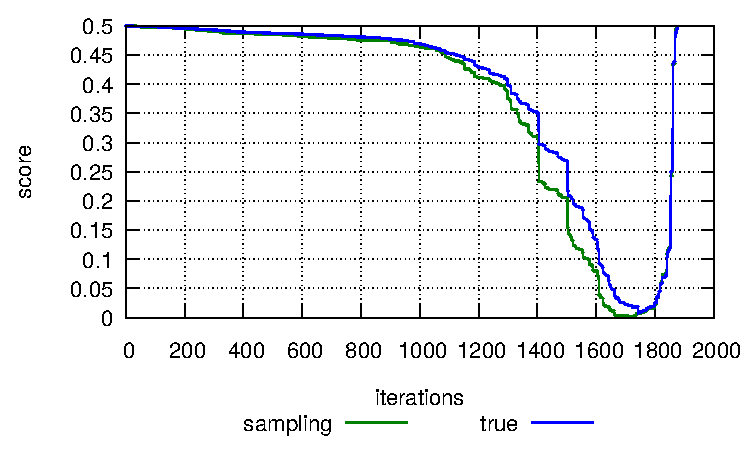
\includegraphics[height=3.2cm, width=4.2cm,valign=t]{figures/plot_real_a.pdf}
        \caption{Average linkage}
    \end{subfigure}
    
    \caption{Publications dataset: Loss reported for every iteration of hierarchical clustering}
    \label{fig:publications}
\end{figure*}

\begin{table}[t]
\centering
\begin{tabular}{ |c || c|c||c|c| } 
 \hline
  & \multicolumn{2}{c||}{\textbf{simulated}} & \multicolumn{2}{|c|}{\textbf{publications}} \\ \hline
Clustering & true-best & sampling-best & true-best & sampling-best \\ \hline
C1 (single) &	0.03612	& 0.03985	&	0.01622 &	0.01824 \\ \hline
C2 (complete) &	0.00730 &	0.01015	&	0.00909	& 0.00912 \\ \hline
C3 (weighted) &	0.00410 &	0.00704	&	0.00511	& 0.00569 \\ \hline
C4 (average) &	0.00395	& 0.00676	& 0.00751	& 0.01686 \\ \hline
\end{tabular}
\caption{Loss values of the true best clustering and the best clustering found by our framework.}
\label{tab:exp3}
\end{table}


We now present the evaluation of our framework on a simulated and a real world dataset.
In Section \ref{sec:exp1} we show that in our framework a relatively small number of samples are enough to accurately estimate the loss of a clustering,
and in Section \ref{sec:exp2} we demonstrate our framework on hierarchical clustering and 
show that the best clustering picked by our approach is very close to the true best clustering.

\subsection{Evaluation setup}
For our evaluation we use two datasets.
First dataset is a simulated dataset of ten thousand strings of length 20 where we simulate a clustering over the set of strings and use it as our ground truth.
We use Jaro distance \cite{jaro1980unimatch} as the distance metric for strings.
To simulate a clustering we generate some seed strings and then for each seed string we generate multiple secondary strings by slightly editing the seed string.
Each cluster of strings resembles a single entity.
Second dataset is a real-world bibliographical information of scientific publications \cite{pubdata}.
The dataset has 1879 publication records with duplicates.
The ground truth of duplicates is available.
To perform clustering on this dataset we first tokenized each publication record and extracted 3-grams from them.
Then, on 3-grams we used Jaccard distance to define distance between two records.
For both the datasets we use ground truth as the oracle that can answer \textit{same-cluster queries}.
We use hierarchical clustering to perform de-duplication on our datasets.
We consider 4 different methods of hierarchical clustering: single linkage (C1), complete linkage (C2), weighted linkage (C3), and average linkage (C4).
%We use the dataset's ground truth to access the quality of any candidate clustering.
%To calculate the true loss of a clustering (i.e. $L_{C^*}(C^*)$) we access all of the ground truth, we also call this as a naive approach.
%Our framework uses only a sample of the ground truth to find the loss of a clustering.
%To judge the performance of our framework we compare its $L_{C^*}(C)$ (normalized correlation loss against the $score$ of the naive approach.

\subsection{Impact of sample size}
\label{sec:exp1}

In this experiment we show that even a small number of samples are enough to estimate the normalized correlation loss ($L_{C^*}(C)$).
We compare the true loss of a clustering ($L_{C^*}(C)$) against the estimated loss $\hat L_{C^*}(C)$.
The true loss is computed by querying every pair $(x_1, x_2) \in X^{[2]}$ against the oracle (ground truth in our case).
We consider four different clusterings, each one picked at random from the four hierarchical clustering methods (C1 - C4).
Table \ref{tab:exp1} and \ref{tab:exp2} reports the loss for simulated and publications dataset, respectively.
For each dataset we increased the number of positive and negative samples and measured the loss.
The table also shows the true loss of the clustering.
It can be seen that the estimated loss calculated by our framework is close to the true loss even with 25 positive samples and 25 negative samples.
In addition to this, the loss does not change much by increasing the number of samples.
Which means that there is no incentive to sample more.
We also show that the number of queries performed by our framework are close to the sample size (as claimed in Thm. \ref{thm:queryComplexity}), which are orders of magnitude less than $O(|X|^2)$.
For example, in the simulated dataset and single linkage clustering (C1) with 25 positive and 25 negative samples our framework performed 51 queries, that means one query was wasted. Similarly, 4 queries were wasted for 100 positive and 100 negative samples, and so on.

\subsection{Hierarchical clustering}
\label{sec:exp2}
In this experiment we demonstrate our framework on four different methods of hierarchical clustering (C1 - C4).
For each clustering, the goal is to find the pruning from the clustering tree that has minimum loss.
We compare the loss of the best clustering found by our framework against the loss of the true-best clustering.
We find the loss of the true-best clustering by performing all $|X|^2$ queries against the ground truth.
In Table \ref{tab:exp3} we report the loss of the best clustering for all four clustering methods and both the datasets.
In all the scenarios the best clustering picked by our framework is very close to the true-best clustering.
The framework used 100 positive and 100 negative samples for this experiment for both the datasets.
In Figures \ref{fig:simulated} and \ref{fig:publications}, we report the loss at every iteration of the hierarchical clustering.
The loss reported by our framework is always close to the true loss of the clustering at every iteration.
Another important point to note is that by only sampling 200 points, we are able to estimate the loss of all the clusterings (or prunings) of the hierarchical clustering tree. 

\ifdefined\COMPLETE
\else
\end{document}
\fi

